\documentclass[a4paper,UTF8]{ctexart}

\usepackage{amsmath, amsthm, amssymb, amsfonts, hyperref, mathrsfs}%美国数学学会的包+?
\usepackage{geometry} %控制界面
\usepackage{bookmark}
\usepackage{fancyhdr} % header & footer
\usepackage{appendix} % 附录
\usepackage{tikz} %作图
\usepackage{graphicx} %插入图片的宏包
\usepackage{float} %设置图片浮动位置的宏包
\usepackage{subfigure} %插入多图时用子图显示的宏包
\usepackage{listings} %引用代码
\usepackage{physics,mathtools} %物理数学工具
\usepackage{comment}
\usepackage{framed}
\geometry{top=2.5cm,bottom=2.5cm,left=2.5cm,right=2.5cm} % 布局要求
\pagestyle{fancy} % fancy分格
\fancyhf{} % 清除所有页眉页脚
\renewcommand\headrulewidth{0.6pt}
\renewcommand\footrulewidth{0.6pt}
\lhead{何金铭 PB21020660$\mid$座位号:2}
\chead{铁磁共振数据处理}
\rhead{\thepage}
\lfoot{2023.5.22}
\rfoot{USTC}
%\bibliographystyle{plain} % 引用样式
\everymath{\displaystyle} % display
%============================================================

\begin{document}

\begin{center}
    \textbf{\Large 铁磁共振数据处理}
    \par \text{\large 何金铭 PB21020660}
\end{center}

\section{测量微波信号频率}

\begin{table}[H]
    \centering
    \begin{tabular}{|c|c|c|c|c|c|c|}
    \hline
        次数 & 1 & 2 & 3 & 4 & 5 & 6 \\ \hline
        波长表读数/mm & 3.549 & 3.539 & 3.545 & 3.545 & 3.541 & 3.545 \\ \hline
        频率/MHz & 8870.25 & 8870.45 & 8870.25 & 8870.25 & 8870.35 & 8870.25 \\ \hline
    \end{tabular}
    \caption{波长表和对应的频率表}
\end{table}

测得波长表读数的平均值为$3.544mm$,频率的平均值为$8870.3$MHz

\section{$I$-$B$曲线的处理}

\subsection{原始数据}

\begin{table}[H]
    \centering
    \begin{tabular}{|c|c|c|c|c|c|c|c|c|c|c|c|}
    \hline
        $I_1/A$ & 1.201 & 1.251 & 1.300 & 1.354 & 1.401 & 1.450 & 1.501 & 1.551 & 1.600 & 1.610 & 1.620 \\ \hline
        $I_2/\mu A$ & 38.5 & 38.3 & 38.0 & 37.8 & 37.3 & 36.6 & 36.0 & 35.0 & 33.2 & 33.0 & 32.5 \\ \hline
        $I_1/A$ & 1.630 & 1.640 & 1.650 & 1.660 & 1.670 & 1.680 & 1.690 & 1.700 & 1.710 & 1.720 & 1.730 \\ \hline
        $I_2/\mu A$ & 32.2 & 31.8 & 31.2 & 30.5 & 30.0 & 29.2 & 28.2 & 27.2 & 26.1 & 25.5 & 24.0 \\ \hline
        $I_1/A$ & 1.740 & 1.750 & 1.760 & 1.770 & 1.784 & 1.790 & 1.800 & 1.811 & 1.821 & 1.831 & 1.840 \\ \hline
        $I_2/\mu A$ & 22.5 & 21.5 & 20.0 & 18.5 & 17.0 & 16.2 & 15.5 & 14.8 & 14.8 & 15.4 & 16.5 \\ \hline
        $I_1/A$ & 1.850 & 1.860 & 1.870 & 1.880 & 1.891 & 1.900 & 1.910 & 1.920 & 1.930 & 1.940 & 1.950 \\ \hline
        $I_2/\mu A$ & 18.2 & 20.0 & 22.5 & 25.5 & 28.0 & 30.5 & 32.5 & 34.2 & 36.5 & 38.0 & 39.5 \\ \hline
        $I_1/A$ & 1.960 & 1.970 & 1.980 & 1.990 & 2.000 & 2.050 & 2.100 & 2.150 &  & ~ & ~ \\ \hline
        $I_2/\mu A$ & 40.5 & 41.5 & 42.3 & 43.0 & 43.5 & 45.5 & 46.2 & 46.5 &  & ~ & ~ \\ \hline
    \end{tabular}
    \caption{B上升时的I-B曲线原始数据记录表}
\end{table}

\begin{table}[H]
    \centering
    \begin{tabular}{|c|c|c|c|c|c|c|c|c|c|c|}
    \hline
        $I_1/A$ & 2.000 & 1.950 & 1.900 & 1.890 & 1.878 & 1.868 & 1.859 & 1.847 & 1.836 & 1.826 \\ \hline
        $I_2/\mu A$ & 45.0 & 42.5 & 36.5 & 34.0 & 32.0 & 29.5 & 26.5 & 23.5 & 20.5 & 18.5 \\ \hline
        $I_1/A$ & 1.816 & 1.807 & 1.797 & 1.786 & 1.776 & 1.765 & 1.756 & 1.742 & 1.735 & 1.725 \\ \hline
        $I_2/\mu A$ & 17.0 & 16.0 & 15.5 & 15.5 & 16.5 & 17.8 & 18.8 & 21.2 & 22.5 & 24.0 \\ \hline
        $I_1/A$ & 1.714 & 1.704 & 1.694 & 1.683 & 1.675 & 1.665 & 1.654 & 1.642 & 1.630 & 1.620 \\ \hline
        $I_2/\mu A$ & 25.8 & 27.5 & 29.0 & 30.5 & 31.5 & 32.5 & 33.5 & 34.5 & 35.5 & 36.5 \\ \hline
        $I_1/A$ & 1.609 & 1.596 & 1.584 & 1.571 & 1.518 & 1.468 & 1.412 & 1.369 & 1.315 & 1.265 \\ \hline
        $I_2/\mu A$ & 37.3 & 38.0 & 38.5 & 39.2 & 41.0 & 42.0 & 43.0 & 43.5 & 44.0 & 44.5 \\ \hline
    \end{tabular}
    \caption{B下降时的I-B曲线原始数据记录表}
\end{table}

\subsection{处理后数据}

\subsubsection{B上升的情况}

\begin{table}[H]
    \centering
    \begin{tabular}{|c|c|c|c|c|c|c|c|c|c|c|c|}
    \hline
        $B/mT$ & 191 & 199 & 207 & 214 & 222 & 230 & 238 & 245 & 253 & 254.6 & 256.2 \\ \hline
        $I/\mu A$ & 38.5 & 38.3 & 38.0 & 37.8 & 37.3 & 36.6 & 36.0 & 35.0 & 33.2 & 33.0 & 32.5 \\ \hline
        $B/mT$ & 257.8 & 259.4 & 261 & 262.6 & 264.2 & 265.8 & 267.4 & 269 & 270.4 & 271.8 & 273.2 \\ \hline
        $I/\mu A$ & 32.2 & 31.8 & 31.2 & 30.5 & 30.0 & 29.2 & 28.2 & 27.2 & 26.1 & 25.5 & 24.0 \\ \hline
        $B/mT$ & 274.6 & 276 & 277.6 & 279.2 & 280.8 & 282.4 & 284 & 285.4 & 286.8 & 288.2 & 289.6 \\ \hline
        $I/\mu A$ & 22.5 & 21.5 & 20.0 & 18.5 & 17.0 & 16.2 & 15.5 & 14.8 & 14.8 & 15.4 & 16.5 \\ \hline
        $B/mT$ & 291 & 292.6 & 294.2 & 295.8 & 297.4 & 299 & 300.4 & 301.8 & 303.2 & 304.6 & 306 \\ \hline
        $I/\mu A$ & 18.2 & 20.0 & 22.5 & 25.5 & 28.0 & 30.5 & 32.5 & 34.2 & 36.5 & 38.0 & 39.5 \\ \hline
        $B/mT$ & 307.6 & 309.2 & 310.8 & 312.4 & 314 & 321 & 329 & 336 &  & ~ & ~ \\ \hline
        $I/\mu A$ & 40.5 & 41.5 & 42.3 & 43.0 & 43.5 & 45.5 & 46.2 & 46.5 &  & ~ & ~ \\ \hline
    \end{tabular}
    \caption{B上升时的I-B曲线数据记录表}
\end{table}

\begin{figure}[H]
    \centering
    \begin{minipage}[b]{0.9\textwidth}
        \centering
        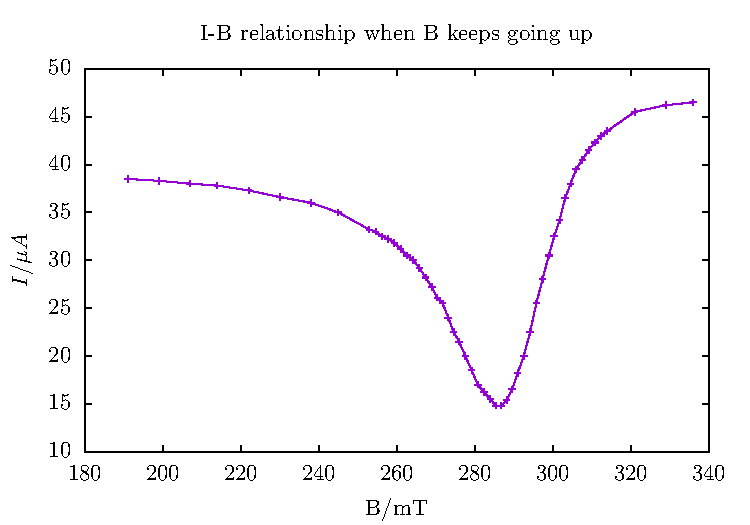
\includegraphics[width=0.8\textwidth]{./f1.pdf}
        \caption{B上升时的I-B曲线}
    \end{minipage}
\end{figure}

\begin{enumerate}
    \item[$I_0$:] 选取$I_0$为左右渐近线值的平均值,$I_0 = \frac{38.5+46.5}{2}\mu A=42.5\mu A$
    \item[$I_r$:] $I_r$为峰谷对应的电流值,$I_r = 14.8\mu A$
\end{enumerate}

计算得$I_{\frac{1}{2}}$为:

\begin{equation}
    I_{\frac{1}{2}} = \frac{2 I_0 I_{r}}{I_0 + I_{r}} = \frac{2 \cdot 42.5 \cdot 14.8}{42.5+14.8}\mu A = 21.9546 \mu A
\end{equation}

通过差值的方法计算得$\Delta B = 17.62 mT$,并且观察得$B_r = 286.1 mT$

计算得朗德因子$g$为:

\begin{equation}
    g = \frac{\gamma \hbar}{\mu_B} = \frac{2\pi \nu}{B_r} \cdot \frac{\hbar}{\mu_B} = \frac{2\pi \cdot 8870.3 MHZ}{286.1 mT} \cdot \frac{1.054 \times 10^{-34}J\cdot s}{9.274 \times 10^{-24} J\cdot T^{-1}} = 2.214
\end{equation}

\subsubsection{B下降的情况}

\begin{table}[H]
    \centering
    \begin{tabular}{|c|c|c|c|c|c|c|c|c|c|c|}
    \hline
        $I_1/A$ & 322 & 314 & 306 & 304.6 & 302.92 & 301.52 & 300.26 & 298.52 & 296.76 & 295.16 \\ \hline
        $I_2/\mu A$ & 45.0 & 42.5 & 36.5 & 34.0 & 32.0 & 29.5 & 26.5 & 23.5 & 20.5 & 18.5 \\ \hline
        $I_1/A$ & 293.56 & 292.12 & 290.52 & 288.76 & 287.16 & 285.4 & 283.96 & 281.88 & 280.9 & 279.5 \\ \hline
        $I_2/\mu A$ & 17.0 & 16.0 & 15.5 & 15.5 & 16.5 & 17.8 & 18.8 & 21.2 & 22.5 & 24.0 \\ \hline
        $I_1/A$ & 277.96 & 276.56 & 275.04 & 273.28 & 272 & 270.4 & 268.64 & 266.72 & 264.8 & 263.2 \\ \hline
        $I_2/\mu A$ & 25.8 & 27.5 & 29.0 & 30.5 & 31.5 & 32.5 & 33.5 & 34.5 & 35.5 & 36.5 \\ \hline
        $I_1/A$ & 261.44 & 259.36 & 257.44 & 255.36 & 246.88 & 238.88 & 229.92 & 223.04 & 215.1 & 207.4 \\ \hline
        $I_2/\mu A$ & 37.3 & 38.0 & 38.5 & 39.2 & 41.0 & 42.0 & 43.0 & 43.5 & 44.0 & 44.5 \\ \hline
    \end{tabular}
    \caption{B下降时的I-B曲线数据记录表}
\end{table}

\begin{figure}[H]
    \centering
    \begin{minipage}[b]{0.9\textwidth}
        \centering
        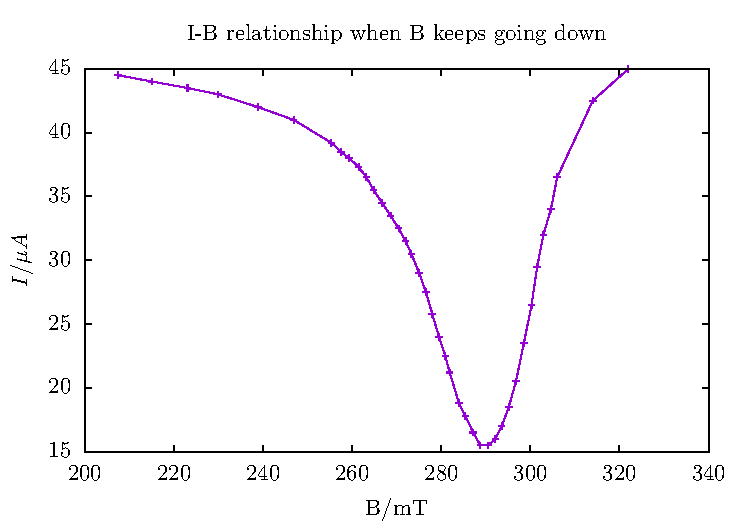
\includegraphics[width=0.8\textwidth]{./f2.pdf}
        \caption{B上升时的I-B曲线}
    \end{minipage}
\end{figure}

\begin{enumerate}
    \item[$I_0$:] 选取$I_0$为左右渐近线值的平均值,$I_0 = \frac{45.0+44.5}{2}\mu A=44.75\mu A$
    \item[$I_r$:] $I_r$为峰谷对应的电流值,$I_r = 15.5\mu A$
\end{enumerate}

计算得$I_{\frac{1}{2}}$为:

\begin{equation}
    I_{\frac{1}{2}} = \frac{2 I_0 I_{r}}{I_0 + I_{r}} = \frac{2 \cdot 44.75 \cdot 15.5}{44.75+15.5}\mu A = 23.0249 \mu A
\end{equation}

通过差值的方法计算得$\Delta B = 17.09 mT$,并且观察得$B_r = 289.64 mT$

计算得朗德因子$g$为:

\begin{equation}
    g = \frac{\gamma \hbar}{\mu_B} = \frac{2\pi \nu}{B_r} \cdot \frac{\hbar}{\mu_B} = \frac{2\pi \cdot 8870.3 MHZ}{289.64 mT} \cdot \frac{1.054 \times 10^{-34}J\cdot s}{9.274 \times 10^{-24} J\cdot T^{-1}} = 2.187
\end{equation}

\subsubsection{总结}

综上:

\begin{equation}
    \Delta B = \frac{\Delta B_1 + \Delta B_2}{2} = \frac{17.62+17.09}{2} mT = 17.36 mT
\end{equation}

\begin{equation}
    g = \frac{g_1 + g_2}{2} = \frac{2.214+2.187}{2} = 2.201
\end{equation}

\section{共振波形图}

\begin{figure}[H]
    \centering
    \begin{minipage}[b]{0.9\textwidth}
        \centering
        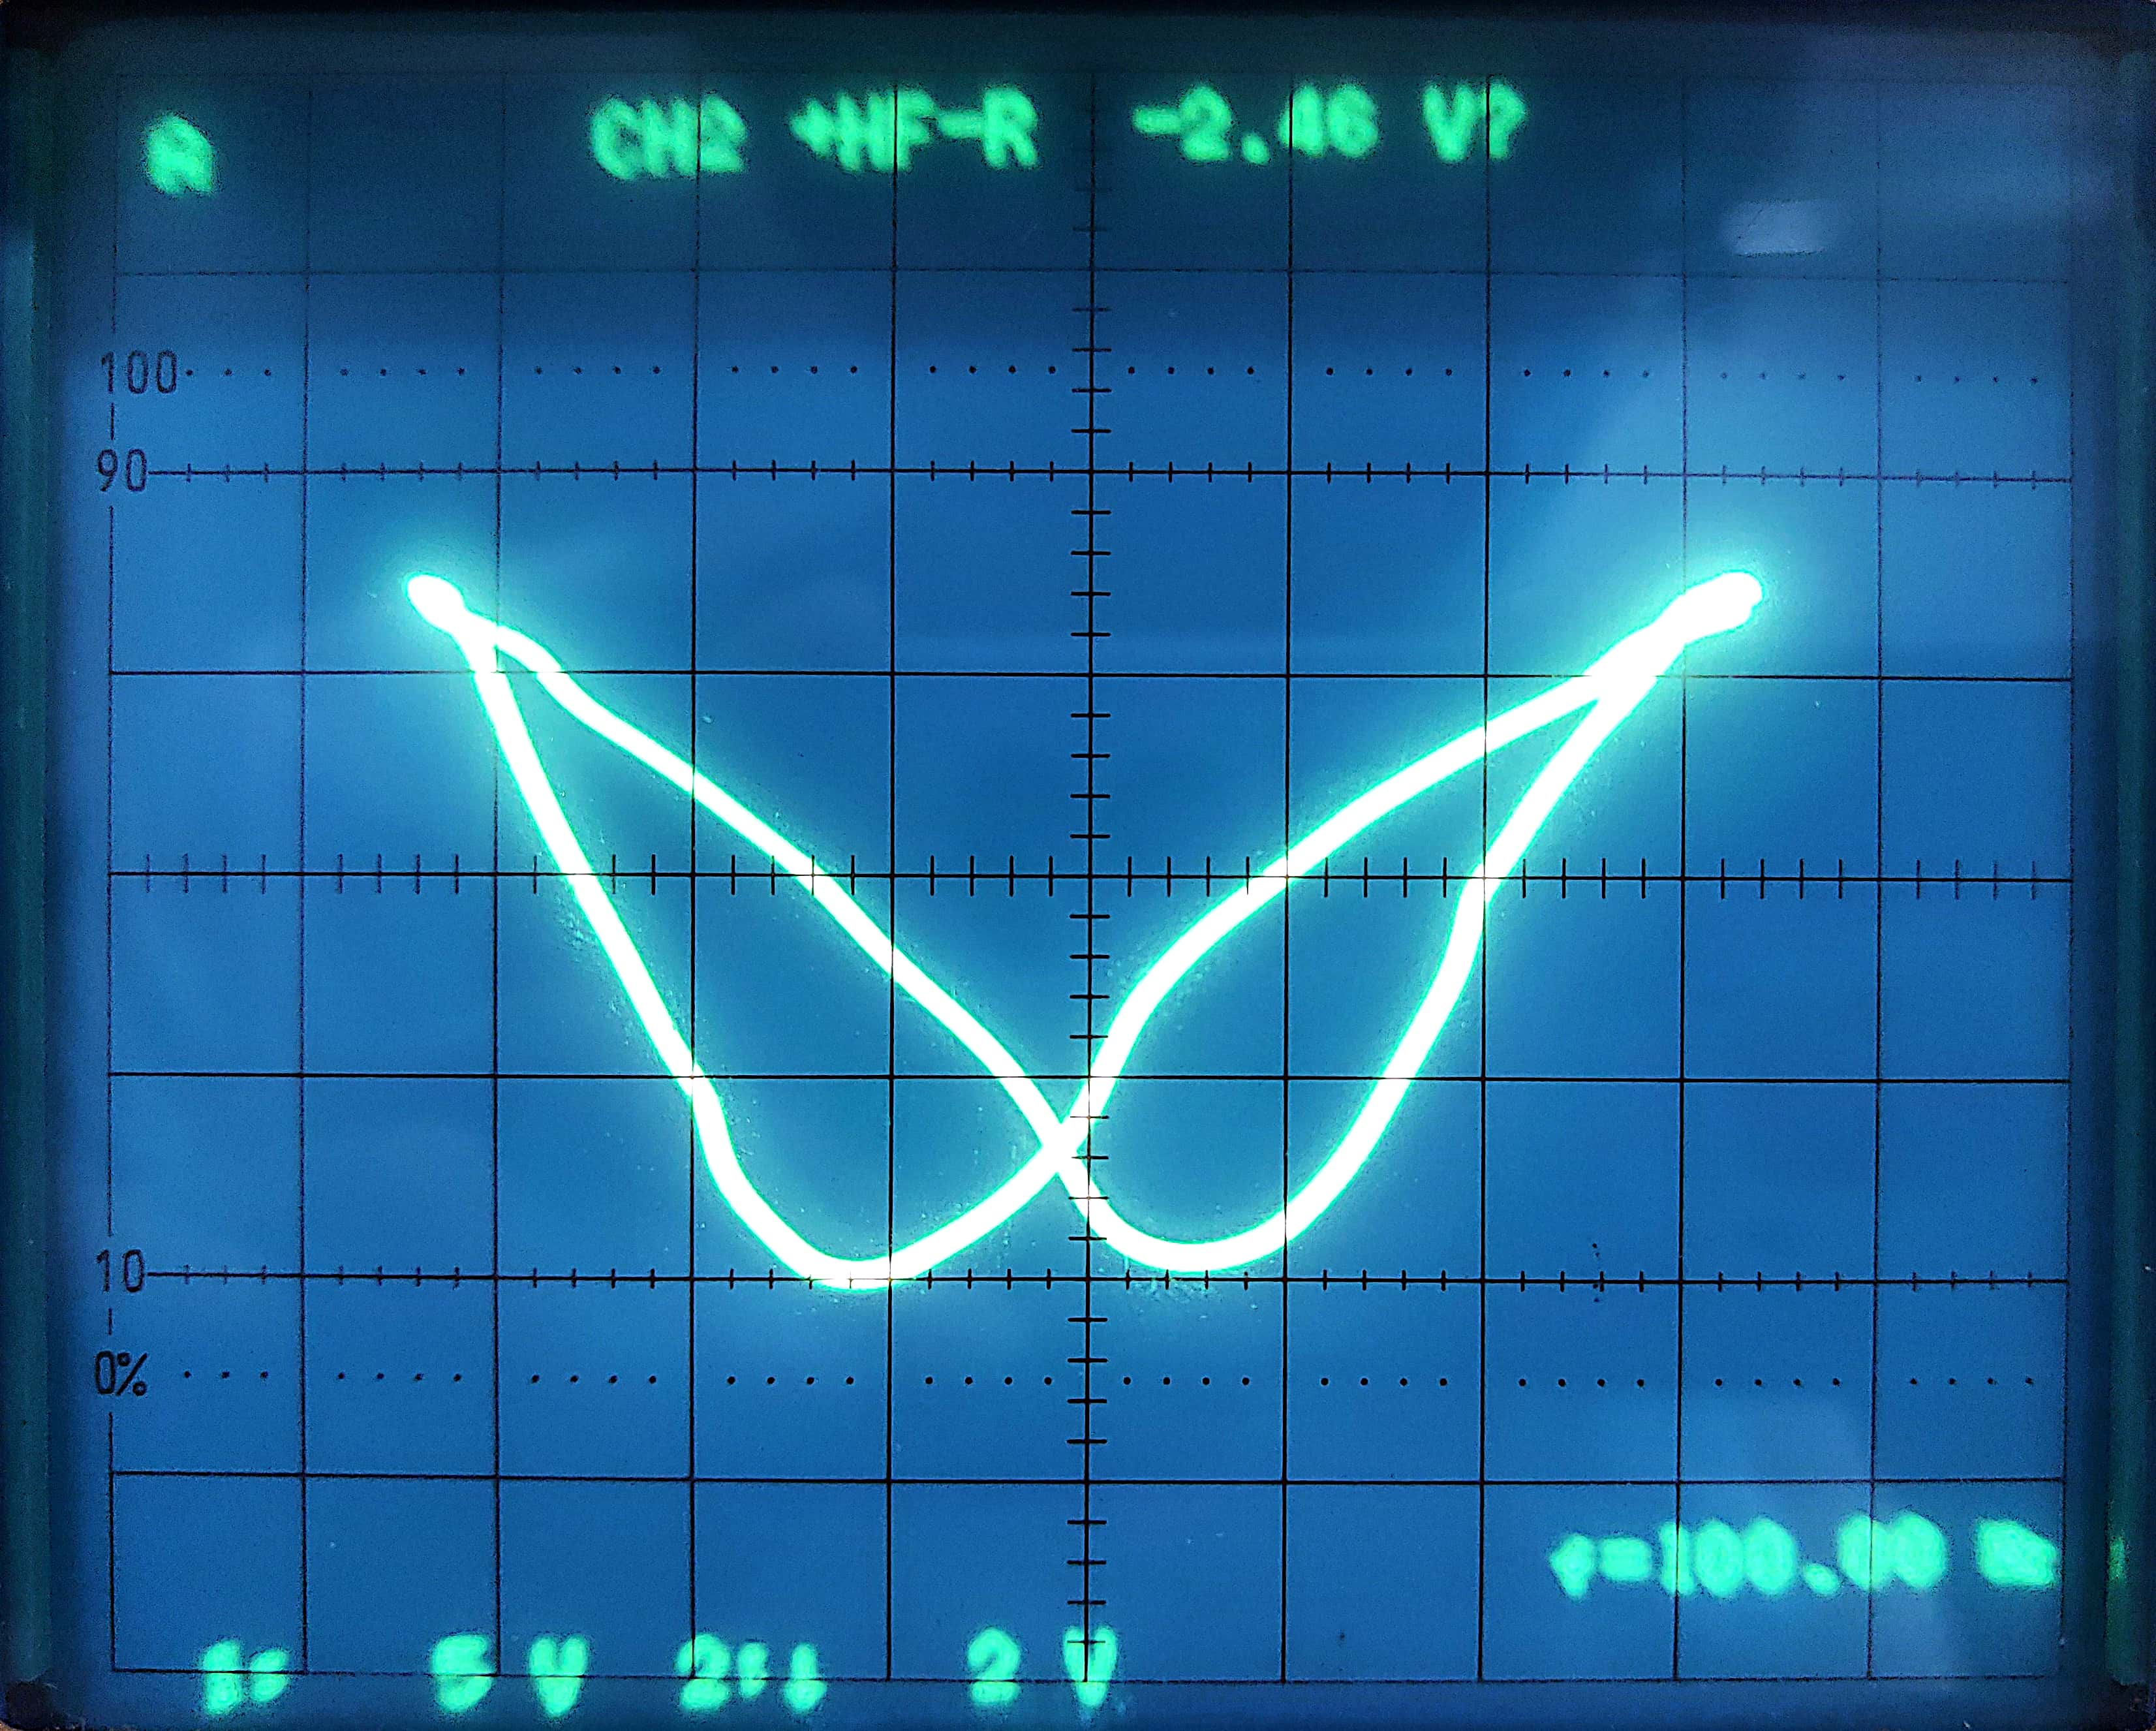
\includegraphics[width=0.7\textwidth]{./fig1.png}
        \caption{用示波器观察的共振波形图}
    \end{minipage}
\end{figure}

X轴代表的是随时间左右震荡的电流信号,反映了B的变化;Y轴代表的是另一个随时间左右震荡的电流信号,反映了I的变化。和上面画的$I$-$B$曲线类似。

\section{思考题}

\subsection*{4. 能否从试验结果曲线,取曲线高度一半处对应的磁场差作为$\Delta B$?为什么?}

不能。因为在实际测量中测的是$I$-$B$曲线,而不是$\mu''$-$B$曲线。而检波电流I在一定条件下与
输出功率$P_{out}$成正比,而$P_{out}$表征的是品质因数$Q_L$的变化,进而反映$\mu''$的变化。
而这几个量之间并不是线性关系,由下式易得:

\begin{equation}
    \Delta (\frac{1}{Q_L}) = 4A\mu'
\end{equation}

\begin{equation}
    P_{out}(\omega_0)=\frac{4P_{in}(\omega_0)}{Q_{e1}Q_{e2}}\cdot Q_L^2
\end{equation}

故不能取曲线高度一半处对应的磁场差作为$\Delta B$。

\end{document}